\PassOptionsToPackage{unicode=true}{hyperref} % options for packages loaded elsewhere
\PassOptionsToPackage{hyphens}{url}
%
\documentclass[ignorenonframetext,]{beamer}
\usepackage{pgfpages}
\setbeamertemplate{caption}[numbered]
\setbeamertemplate{caption label separator}{: }
\setbeamercolor{caption name}{fg=normal text.fg}
\beamertemplatenavigationsymbolsempty
% Prevent slide breaks in the middle of a paragraph:
\widowpenalties 1 10000
\raggedbottom
\setbeamertemplate{part page}{
\centering
\begin{beamercolorbox}[sep=16pt,center]{part title}
  \usebeamerfont{part title}\insertpart\par
\end{beamercolorbox}
}
\setbeamertemplate{section page}{
\centering
\begin{beamercolorbox}[sep=12pt,center]{part title}
  \usebeamerfont{section title}\insertsection\par
\end{beamercolorbox}
}
\setbeamertemplate{subsection page}{
\centering
\begin{beamercolorbox}[sep=8pt,center]{part title}
  \usebeamerfont{subsection title}\insertsubsection\par
\end{beamercolorbox}
}
\AtBeginPart{
  \frame{\partpage}
}
\AtBeginSection{
  \ifbibliography
  \else
    \frame{\sectionpage}
  \fi
}
\AtBeginSubsection{
  \frame{\subsectionpage}
}
\usepackage{lmodern}
\usepackage{amssymb,amsmath}
\usepackage{ifxetex,ifluatex}
\usepackage{fixltx2e} % provides \textsubscript
\ifnum 0\ifxetex 1\fi\ifluatex 1\fi=0 % if pdftex
  \usepackage[T1]{fontenc}
  \usepackage[utf8]{inputenc}
  \usepackage{textcomp} % provides euro and other symbols
\else % if luatex or xelatex
  \usepackage{unicode-math}
  \defaultfontfeatures{Ligatures=TeX,Scale=MatchLowercase}
\fi
\usetheme[]{CambridgeUS}
\usecolortheme{beaver}
\usefonttheme{structurebold}
% use upquote if available, for straight quotes in verbatim environments
\IfFileExists{upquote.sty}{\usepackage{upquote}}{}
% use microtype if available
\IfFileExists{microtype.sty}{%
\usepackage[]{microtype}
\UseMicrotypeSet[protrusion]{basicmath} % disable protrusion for tt fonts
}{}
\IfFileExists{parskip.sty}{%
\usepackage{parskip}
}{% else
\setlength{\parindent}{0pt}
\setlength{\parskip}{6pt plus 2pt minus 1pt}
}
\usepackage{hyperref}
\hypersetup{
            pdftitle={1. Computer Systems - Course Overview},
            pdfauthor={CT1100 - J. Duggan},
            pdfborder={0 0 0},
            breaklinks=true}
\urlstyle{same}  % don't use monospace font for urls
\newif\ifbibliography
\usepackage{color}
\usepackage{fancyvrb}
\newcommand{\VerbBar}{|}
\newcommand{\VERB}{\Verb[commandchars=\\\{\}]}
\DefineVerbatimEnvironment{Highlighting}{Verbatim}{commandchars=\\\{\}}
% Add ',fontsize=\small' for more characters per line
\usepackage{framed}
\definecolor{shadecolor}{RGB}{248,248,248}
\newenvironment{Shaded}{\begin{snugshade}}{\end{snugshade}}
\newcommand{\AlertTok}[1]{\textcolor[rgb]{0.94,0.16,0.16}{#1}}
\newcommand{\AnnotationTok}[1]{\textcolor[rgb]{0.56,0.35,0.01}{\textbf{\textit{#1}}}}
\newcommand{\AttributeTok}[1]{\textcolor[rgb]{0.77,0.63,0.00}{#1}}
\newcommand{\BaseNTok}[1]{\textcolor[rgb]{0.00,0.00,0.81}{#1}}
\newcommand{\BuiltInTok}[1]{#1}
\newcommand{\CharTok}[1]{\textcolor[rgb]{0.31,0.60,0.02}{#1}}
\newcommand{\CommentTok}[1]{\textcolor[rgb]{0.56,0.35,0.01}{\textit{#1}}}
\newcommand{\CommentVarTok}[1]{\textcolor[rgb]{0.56,0.35,0.01}{\textbf{\textit{#1}}}}
\newcommand{\ConstantTok}[1]{\textcolor[rgb]{0.00,0.00,0.00}{#1}}
\newcommand{\ControlFlowTok}[1]{\textcolor[rgb]{0.13,0.29,0.53}{\textbf{#1}}}
\newcommand{\DataTypeTok}[1]{\textcolor[rgb]{0.13,0.29,0.53}{#1}}
\newcommand{\DecValTok}[1]{\textcolor[rgb]{0.00,0.00,0.81}{#1}}
\newcommand{\DocumentationTok}[1]{\textcolor[rgb]{0.56,0.35,0.01}{\textbf{\textit{#1}}}}
\newcommand{\ErrorTok}[1]{\textcolor[rgb]{0.64,0.00,0.00}{\textbf{#1}}}
\newcommand{\ExtensionTok}[1]{#1}
\newcommand{\FloatTok}[1]{\textcolor[rgb]{0.00,0.00,0.81}{#1}}
\newcommand{\FunctionTok}[1]{\textcolor[rgb]{0.00,0.00,0.00}{#1}}
\newcommand{\ImportTok}[1]{#1}
\newcommand{\InformationTok}[1]{\textcolor[rgb]{0.56,0.35,0.01}{\textbf{\textit{#1}}}}
\newcommand{\KeywordTok}[1]{\textcolor[rgb]{0.13,0.29,0.53}{\textbf{#1}}}
\newcommand{\NormalTok}[1]{#1}
\newcommand{\OperatorTok}[1]{\textcolor[rgb]{0.81,0.36,0.00}{\textbf{#1}}}
\newcommand{\OtherTok}[1]{\textcolor[rgb]{0.56,0.35,0.01}{#1}}
\newcommand{\PreprocessorTok}[1]{\textcolor[rgb]{0.56,0.35,0.01}{\textit{#1}}}
\newcommand{\RegionMarkerTok}[1]{#1}
\newcommand{\SpecialCharTok}[1]{\textcolor[rgb]{0.00,0.00,0.00}{#1}}
\newcommand{\SpecialStringTok}[1]{\textcolor[rgb]{0.31,0.60,0.02}{#1}}
\newcommand{\StringTok}[1]{\textcolor[rgb]{0.31,0.60,0.02}{#1}}
\newcommand{\VariableTok}[1]{\textcolor[rgb]{0.00,0.00,0.00}{#1}}
\newcommand{\VerbatimStringTok}[1]{\textcolor[rgb]{0.31,0.60,0.02}{#1}}
\newcommand{\WarningTok}[1]{\textcolor[rgb]{0.56,0.35,0.01}{\textbf{\textit{#1}}}}
\usepackage{longtable,booktabs}
\usepackage{caption}
% These lines are needed to make table captions work with longtable:
\makeatletter
\def\fnum@table{\tablename~\thetable}
\makeatother
\usepackage{graphicx,grffile}
\makeatletter
\def\maxwidth{\ifdim\Gin@nat@width>\linewidth\linewidth\else\Gin@nat@width\fi}
\def\maxheight{\ifdim\Gin@nat@height>\textheight\textheight\else\Gin@nat@height\fi}
\makeatother
% Scale images if necessary, so that they will not overflow the page
% margins by default, and it is still possible to overwrite the defaults
% using explicit options in \includegraphics[width, height, ...]{}
\setkeys{Gin}{width=\maxwidth,height=\maxheight,keepaspectratio}
\setlength{\emergencystretch}{3em}  % prevent overfull lines
\providecommand{\tightlist}{%
  \setlength{\itemsep}{0pt}\setlength{\parskip}{0pt}}
\setcounter{secnumdepth}{0}

% set default figure placement to htbp
\makeatletter
\def\fps@figure{htbp}
\makeatother


\title{1. Computer Systems - Course Overview}
\author{CT1100 - J. Duggan}
\date{}

\begin{document}
\frame{\titlepage}

\begin{frame}{CT1100 Overview}
\protect\hypertarget{ct1100-overview}{}

\begin{itemize}
\tightlist
\item
  Exploring the essential building blocks of the information age
\item
  Semester 1 (J. Duggan)

  \begin{itemize}
  \tightlist
  \item
    Data
  \item
    Hardware
  \end{itemize}
\item
  Semester 2 (M. Rezaei)

  \begin{itemize}
  \tightlist
  \item
    Software
  \item
    Networks
  \end{itemize}
\item
  Module Information

  \begin{itemize}
  \tightlist
  \item
    Compulsory for all first year BA students taking IT as a subject
  \item
    Labs from week 4 (1 hour per week, 3 time slots)
  \item
    Worth 5 ECTS in credit
  \item
    Covered in Semester 1 and Semester 2
  \item
    Continuous Assessment (MCQ tests, Assigments, Lab Exam)
  \item
    \url{https://github.com/JimDuggan/CT1100}
  \end{itemize}
\end{itemize}

\end{frame}

\begin{frame}{Overall Plan (Semester 1)}
\protect\hypertarget{overall-plan-semester-1}{}

\begin{longtable}[]{@{}cl@{}}
\toprule
Lecture(s) & Topic\tabularnewline
\midrule
\endhead
1 & Course Introduction\tabularnewline
2 & The Processing Cycle and Binary Data\tabularnewline
3 & Data in R with Atomic Vectors\tabularnewline
4 & The CRAN Library and Calling Functions in R\tabularnewline
5 & Tidy Data and Data Frames\tabularnewline
6-7 & \textbf{ggplot2} - A Grammar of Graphics\tabularnewline
8-10 & \textbf{dplyr} - A Grammar of Data Manipulation\tabularnewline
11-12 & Introduction to Hardware\tabularnewline
\bottomrule
\end{longtable}

\end{frame}

\begin{frame}{The Processing Cycle in Computing}
\protect\hypertarget{the-processing-cycle-in-computing}{}

\begin{itemize}
\tightlist
\item
  Input, Process, Output key stages in computing
\item
  Image recognition

  \begin{itemize}
  \tightlist
  \item
    Input (a photo)
  \item
    Process (an algorithm)
  \item
    Output (a name)
  \end{itemize}
\end{itemize}

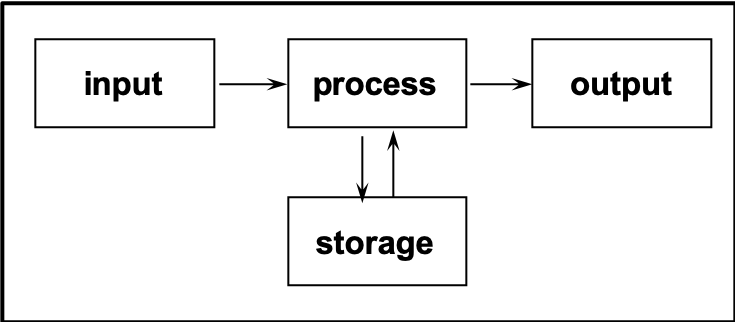
\includegraphics[width=0.7\linewidth]{images/01 Processing}

\end{frame}

\begin{frame}{Sample Input Data (Match Events)}
\protect\hypertarget{sample-input-data-match-events}{}

\begin{longtable}[]{@{}rllllrr@{}}
\toprule
Time & Team & Scorer & From & Type & Points & Score\tabularnewline
\midrule
\endhead
1 & Dublin & Paul Mannion & Play & Point & 1 & 1\tabularnewline
2 & Kerry & Sean O'Shea & Play & Point & 1 & 1\tabularnewline
3 & Dublin & Dean Rock & Play & Point & 1 & 2\tabularnewline
4 & Dublin & Dean Rock & Free & Point & 1 & 3\tabularnewline
10 & Kerry & David Clifford & Play & Point & 1 & 2\tabularnewline
13 & Kerry & Sean O'Shea & FortyFive & Point & 1 & 3\tabularnewline
14 & Kerry & Stephen O'Brien & Play & Point & 1 & 4\tabularnewline
16 & Dublin & Paul Mannion & Play & Point & 1 & 4\tabularnewline
18 & Kerry & Sean O'Shea & Free & Point & 1 & 5\tabularnewline
19 & Dublin & Jack McCaffrey & Play & Goal & 3 & 7\tabularnewline
\bottomrule
\end{longtable}

\end{frame}

\begin{frame}[fragile]{Processing - Summarising the Data}
\protect\hypertarget{processing---summarising-the-data}{}

\begin{verbatim}
## # A tibble: 10 x 3
## # Groups:   Team [2]
##    Team   Scorer           Points
##    <chr>  <chr>             <dbl>
##  1 Dublin Dean Rock            10
##  2 Dublin Jack McCaffrey        6
##  3 Dublin Paul Mannion          2
##  4 Dublin Con O'Callaghan       1
##  5 Kerry  Sean O'Shea          10
##  6 Kerry  Killian Spillane      4
##  7 Kerry  David Clifford        2
##  8 Kerry  Gavin Crowley         1
##  9 Kerry  Stephen O'Brien       1
## 10 Kerry  Tommy Walsh           1
\end{verbatim}

\end{frame}

\begin{frame}[fragile]{Processing - Analysing the Scores}
\protect\hypertarget{processing---analysing-the-scores}{}

\begin{verbatim}
## # A tibble: 6 x 3
## # Groups:   Team [2]
##   Team   From      Points
##   <chr>  <chr>      <dbl>
## 1 Dublin Play          12
## 2 Dublin Free           6
## 3 Dublin FortyFive      1
## 4 Kerry  Play          12
## 5 Kerry  Free           4
## 6 Kerry  FortyFive      3
\end{verbatim}

\end{frame}

\begin{frame}[fragile]{Processing - Before the 34th Minute}
\protect\hypertarget{processing---before-the-34th-minute}{}

\begin{verbatim}
## # A tibble: 6 x 3
## # Groups:   Team [2]
##   Team   From      Points
##   <chr>  <chr>      <dbl>
## 1 Dublin Play           8
## 2 Dublin Free           3
## 3 Dublin FortyFive      1
## 4 Kerry  Free           3
## 5 Kerry  Play           3
## 6 Kerry  FortyFive      1
\end{verbatim}

\end{frame}

\begin{frame}[fragile]{Processing - After the 34th Minute}
\protect\hypertarget{processing---after-the-34th-minute}{}

\begin{verbatim}
## # A tibble: 5 x 3
## # Groups:   Team [2]
##   Team   From      Points
##   <chr>  <chr>      <dbl>
## 1 Dublin Play           4
## 2 Dublin Free           3
## 3 Kerry  Play           9
## 4 Kerry  FortyFive      2
## 5 Kerry  Free           1
\end{verbatim}

\end{frame}

\begin{frame}{Processing - Visualising the Data}
\protect\hypertarget{processing---visualising-the-data}{}

\includegraphics{overview_files/figure-beamer/unnamed-chunk-7-1.pdf}

\end{frame}

\begin{frame}[fragile]{Data processing in R}
\protect\hypertarget{data-processing-in-r}{}

\begin{Shaded}
\begin{Highlighting}[]
\NormalTok{x <-}\StringTok{ }\KeywordTok{c}\NormalTok{(}\DecValTok{3}\NormalTok{, }\DecValTok{4}\NormalTok{, }\DecValTok{5}\NormalTok{, }\DecValTok{6}\NormalTok{, }\DecValTok{7}\NormalTok{)}
\NormalTok{x}
\end{Highlighting}
\end{Shaded}

\begin{verbatim}
## [1] 3 4 5 6 7
\end{verbatim}

\begin{Shaded}
\begin{Highlighting}[]
\NormalTok{x[}\DecValTok{1}\OperatorTok{:}\DecValTok{2}\NormalTok{]}
\end{Highlighting}
\end{Shaded}

\begin{verbatim}
## [1] 3 4
\end{verbatim}

\begin{Shaded}
\begin{Highlighting}[]
\KeywordTok{sum}\NormalTok{(x)}
\end{Highlighting}
\end{Shaded}

\begin{verbatim}
## [1] 25
\end{verbatim}

\begin{Shaded}
\begin{Highlighting}[]
\KeywordTok{mean}\NormalTok{(x)}
\end{Highlighting}
\end{Shaded}

\begin{verbatim}
## [1] 5
\end{verbatim}

\begin{Shaded}
\begin{Highlighting}[]
\NormalTok{x }\OperatorTok{>}\StringTok{ }\DecValTok{5}
\end{Highlighting}
\end{Shaded}

\begin{verbatim}
## [1] FALSE FALSE FALSE  TRUE  TRUE
\end{verbatim}

\end{frame}

\begin{frame}{Setup an Account on rstudio.cloud}
\protect\hypertarget{setup-an-account-on-rstudio.cloud}{}


\includegraphics[width=1\linewidth]{images/02 RStudio Create}

\end{frame}

\begin{frame}{Create a project}
\protect\hypertarget{create-a-project}{}

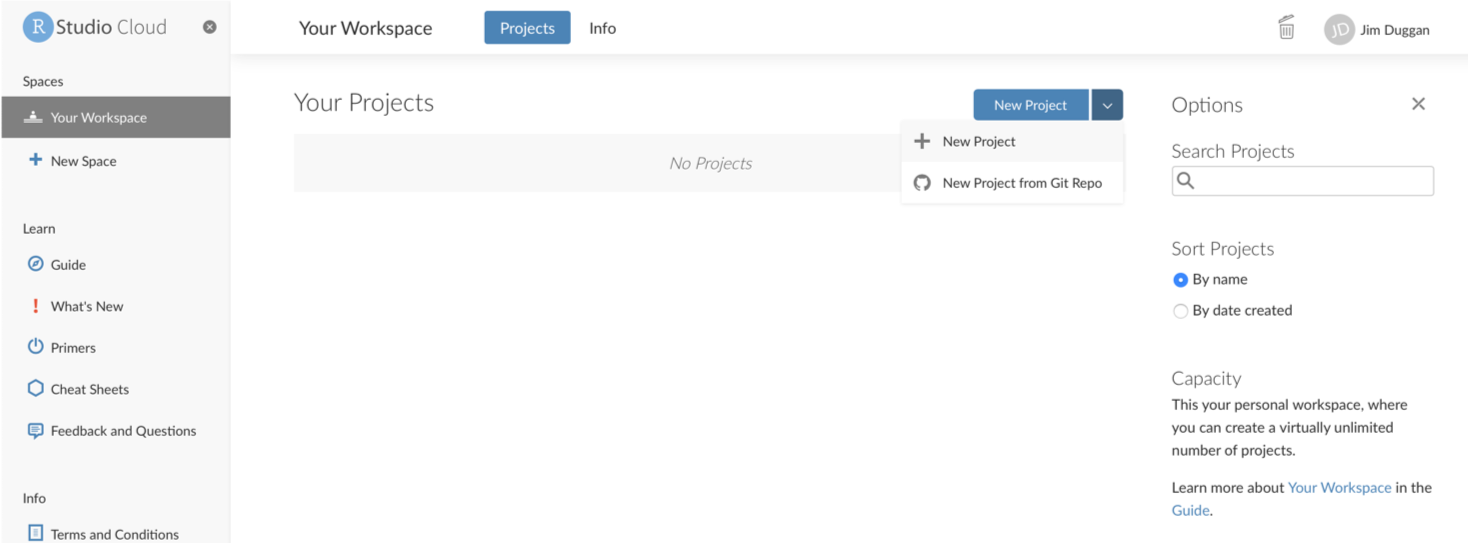
\includegraphics[width=1\linewidth]{images/03 RStudioWorkspace}

\end{frame}

\begin{frame}{RStudio ready for use}
\protect\hypertarget{rstudio-ready-for-use}{}

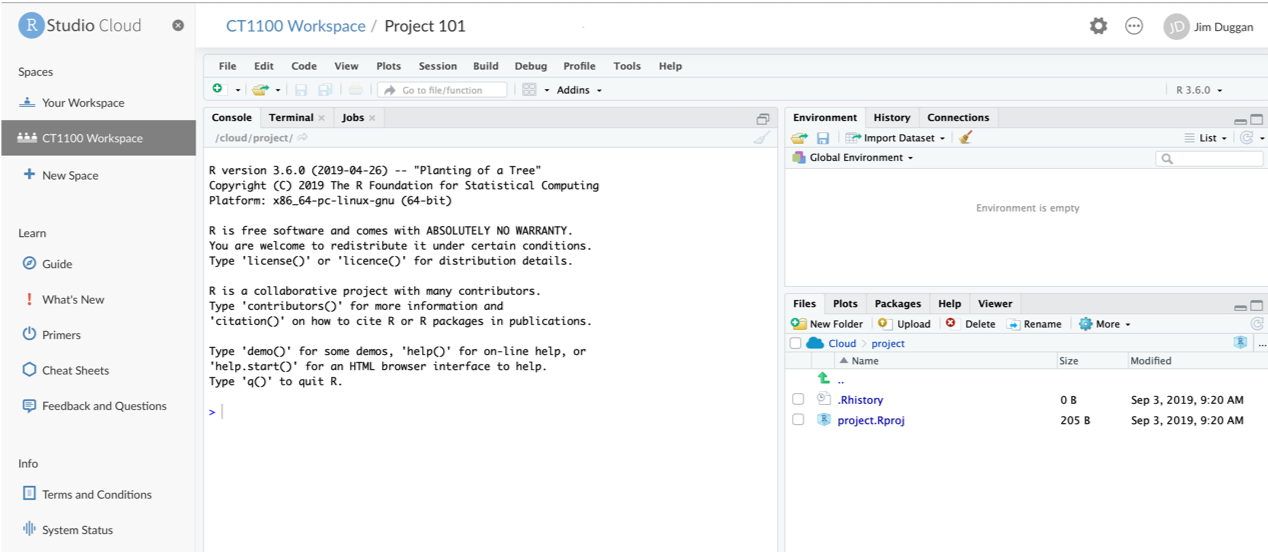
\includegraphics[width=1\linewidth]{images/04 My Project}

\end{frame}

\begin{frame}{Run code in console.}
\protect\hypertarget{run-code-in-console.}{}

\begin{itemize}
\tightlist
\item
  x is data!
\item
  R allows you process the data with function calls
\end{itemize}

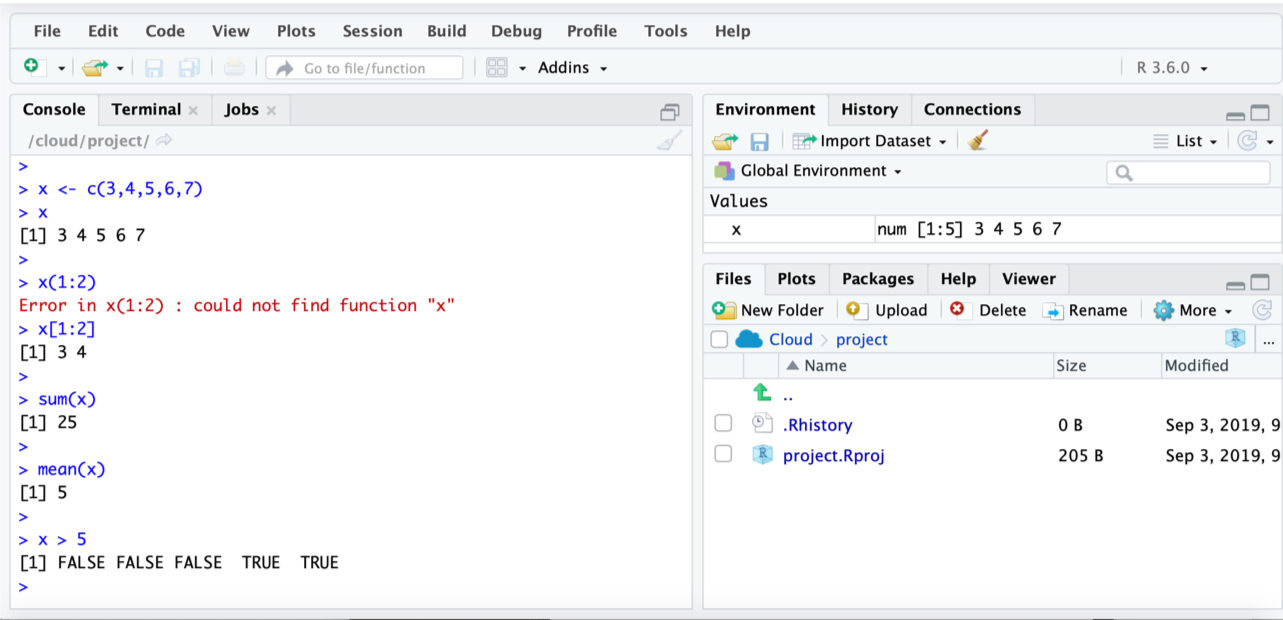
\includegraphics[width=1\linewidth]{images/05 Run Code}

\end{frame}

\begin{frame}{Challange 1.1 - Replicate the following in RStudio Cloud}
\protect\hypertarget{challange-1.1---replicate-the-following-in-rstudio-cloud}{}

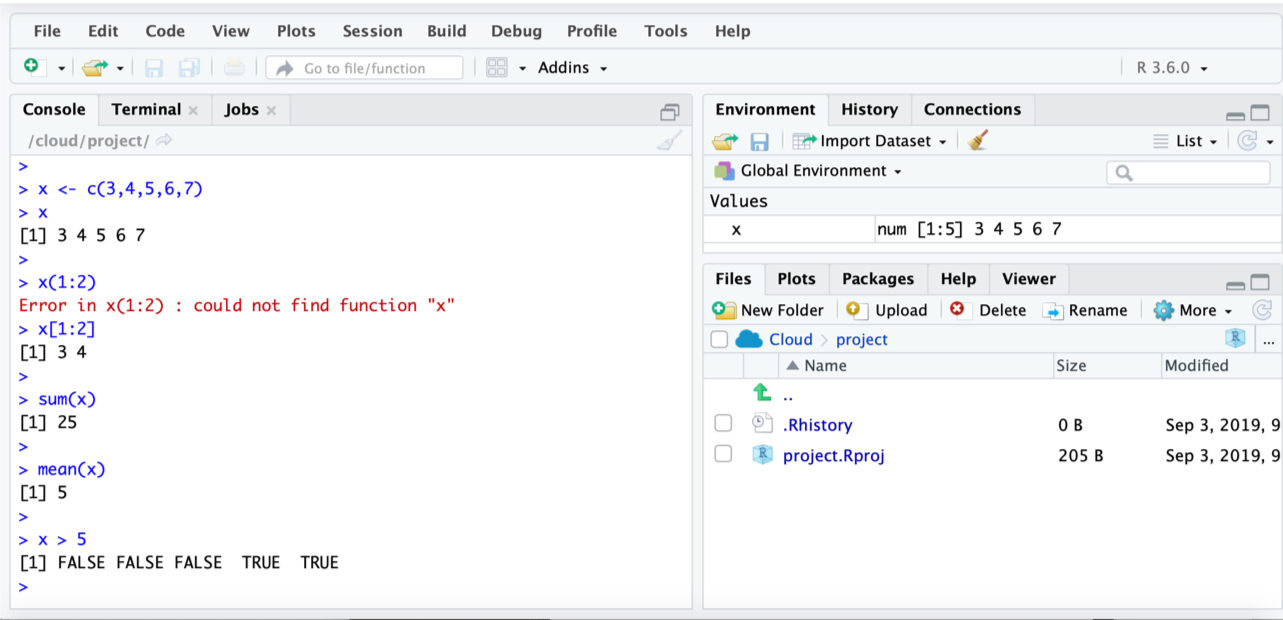
\includegraphics[width=1\linewidth]{images/05 Run Code}

\end{frame}

\begin{frame}{Summary}
\protect\hypertarget{summary}{}

\begin{itemize}
\tightlist
\item
  Welcome to CT1100
\item
  Semester 1

  \begin{itemize}
  \tightlist
  \item
    Practical focus - understanding and manipulating data
  \item
    Using RStudio Cloud
  \end{itemize}
\item
  Next Week

  \begin{itemize}
  \tightlist
  \item
    Input - Process - Output
  \item
    Binary data
  \item
    More on R (atomic vectors)
  \end{itemize}
\end{itemize}

\includegraphics{overview_files/figure-beamer/unnamed-chunk-14-1.pdf}

\end{frame}

\end{document}
